\section{Behavioural Model}
\label{sec:conceptual-behavioral}

The Behavioural Model is the second part of the XRM Conceptual Model. It mainly describes two primitives for creating interactions between the Actors that are part of the experience: User Actions and Effects, detailed later in this section. \\
The aim of the Behavioural Model is to describe the User Actions, actions performed by the user, associated with each of the different types of Non-Human Actor. The Effect, on the other hand, is a perceptible phenomenon that in our model is described to reveal the result of the interaction. 
The Actors depicted in the Structural Model (\autoref{sec:conceptual-structural}) were viewed as static entities. Our approach to behavioural modelling aims to consider Actors as active components, whose behaviour is determined by the actions they execute and the effects they generate on themselves or on other Actors. 
With this in mind we can redefine Actors from a behavior-driven perspective: 
\begin{itemize}
    \item \textbf{Human Actor}: The user who interacts through user actions in order to accomplish a task. It is not taken for granted that the user dealing with the Non-Human Actor concerned has a medium-high level of expertise with technology. The choice of the most intuitive User Action to obtain a given performance is left to the discretion of the designer, who must take into account the average target of users for each experience. 
    \item \textbf{Non-Human Actor}: The actors involved in the XR experience that are reacting to User Actions or events generated by the system. Non-Human Actors include the entire hierarchical structure consisting of Physical Components, the Environment and the Virtual Objects inhabiting it.  It may assume a dual identity role depending on the unit in which it is considered; in some cases it participates, in others it implements the interaction, without excluding that it may embody both at the same time. 
\end{itemize}

\subsection*{User Actions}

User Actions are the actions that the Human Actor performs on the Non-Human Actor involved in accomplishing the task. The Non-Human Actor that participates in the action initiated by the user is called \emph{Target}.
Each User Action corresponds to an event that triggers the interaction. The Actor that can execute User Actions is always and only the Human Actor.

For example, the visitor who uses a visor in a museum is a Human Actor, as much as the tour guide who accompanies him in the VR experience; however, the virtual character of the ancient Greek orator who speaks to the user to introduce the experience, is not an Actor with User Actions.

The main purpose of each User Action is to describe what the Human Actor can perform in order to interact with a certain element, the Target, to obtain a precise reaction which is the one foreseen by the experience model. The decision to involve certain actions, in order to achieve a certain goal, is obviously up to the designer who at the time of creation includes one or more User Actions, so as to allow the user to have different ways to achieve the same desired result. As a consequence, this increases the probability that the model thought by the designer coincides with that perceived by the user, therefore proving that the proposed model has a high level of usability and efficiency. 

The details of how the reaction is triggered are not included in the predefined User Action. The User Actions represent an atomic unit which in the field of software engineering can be associated with library functions, used as a single component in a more complex mechanism whose participants are the user and the Target. 
This makes it possible to apply the concept of re-usability to the conceptual model which was not widely used in the models previously analysed, i.e. the possibility of adding or removing User Actions without affecting the logic of interaction. It is assumed, of course, that the designer chooses among the possible actions the ones supported by the technology involved. For example, it is not possible to tap on an identifiable element such as the QR Code. We do not exclude that the model may include many more technologies and consequently different interaction methods in the future, so the range of possible actions is open to new additions. However, for now, we have encapsulated the main and most common actions the user might perform in an XR experience.
The following are the User Actions identified for this model in the \autoref{tab:BMUserActions}.

\begin{table}[H]
\centering
\begin{tabular}{|l|l|l|}
\hline
\multicolumn{3}{|l|}{\textbf{User Actions}}                                                                                                                      \\ \hline
Tap, Press, Click &
   &
  \begin{tabular}[c]{@{}l@{}}The user through these gestures acts on\\  Physical Components or Virtual Objects, \\ e.g. to navigate, select, show, hide etc.\end{tabular} \\ \hline
\multicolumn{2}{|l|}{Swipe}             & \begin{tabular}[c]{@{}l@{}}The user moves a finger or a hand across\\  a Virtual Object.\end{tabular}                  \\ \hline
\multicolumn{3}{|l|}{Manipulation is described by 3 main types of  User Action:}                                                                                 \\ \hline
              & Drag and Drop           & \begin{tabular}[c]{@{}l@{}}The user can move Virtual Objects \\  from point A to point B.\end{tabular}                 \\ \hline
              & Pinch                   & \begin{tabular}[c]{@{}l@{}}The user can grab Virtual Objects to\\  change their size.\end{tabular}                     \\ \hline
              & Rotate                  & \begin{tabular}[c]{@{}l@{}}The user can turn the Virtual Objects \\ according to the allowed orientation.\end{tabular} \\ \hline
\multicolumn{2}{|l|}{Speak}             & \begin{tabular}[c]{@{}l@{}}The user communicates with the Device \\ through voice commands.\end{tabular}               \\ \hline
\multicolumn{2}{|l|}{Frame} &
  \begin{tabular}[c]{@{}l@{}}The user captures an identifiable element, \\ a Physical Component, through the Device.\end{tabular} \\ \hline
\multicolumn{2}{|l|}{Walk in}           & \begin{tabular}[c]{@{}l@{}}The user moves closer Environments or \\ their Virtual Objects.\end{tabular}                \\ \hline
\multicolumn{2}{|l|}{Walk out}          & \begin{tabular}[c]{@{}l@{}}The user moves away from the Environments \\ or their Virtual Objects.\end{tabular}         \\ \hline
\multicolumn{2}{|l|}{Look around} &
  \begin{tabular}[c]{@{}l@{}}The user moves their gaze, changing the field\\  of view of the 360° Video Environment.\end{tabular} \\ \hline
\multicolumn{2}{|l|}{Gaze In and Dwell} & \begin{tabular}[c]{@{}l@{}}The user looks at a Virtual Object for a certain \\ amount of time.\end{tabular}            \\ \hline
\multicolumn{2}{|l|}{Gaze out}          & \begin{tabular}[c]{@{}l@{}}The user looks away from a Virtual Object\\  within a certain amount of time.\end{tabular}  \\ \hline
\end{tabular}
\caption{Behavioural Model - User Actions}
\label{tab:BMUserActions}
\end{table}

\subsection*{Effect}

The effect is seen as the change of a structural property of an \emph{Actuator} (\autoref{fig:EffectBlock}).

The Actuator is represented by one or more Non-Human Actors on which the generated effect is perceived.
If the User Action is the event that triggers the interaction, the Effect is the reaction to it by one or more Actuators. In some cases, however, it is the system that causes a certain Effect. The next section will clarify this concept. The Effects that can be generated are innumerable, therefore we have selected a few that we consider to be the most important. Below are some examples of Effects:

\begin{table}[H]
\centering
\begin{tabular}{|l|l|}
\hline
\multicolumn{2}{|l|}{\textbf{Effects}}                                                                                                     \\ \hline
Show &
  \begin{tabular}[c]{@{}l@{}}One (or more) Environment or one (or more)\\  of its Virtual Objects becomes visible to the user.\end{tabular} \\ \hline
Hide &
  \begin{tabular}[c]{@{}l@{}}One (or more) Environment or one (or more) \\ of its Virtual Objects is hidden from the user.\end{tabular} \\ \hline
Change User View &
  \begin{tabular}[c]{@{}l@{}}The segment of the 360° Video Environment, \\ visible to the user, is changed.\end{tabular} \\ \hline
Screenshot Acquisition & The screenshot taken is captured by the Device.                                                                   \\ \hline
Recording Acquisition  & The video recording is taken over by the Device.                                                                  \\ \hline
Acquired Element Saved & \begin{tabular}[c]{@{}l@{}}The screenshot or video recording is saved to \\ the Device memory.\end{tabular}       \\ \hline
Speech To Text         & \begin{tabular}[c]{@{}l@{}}The Device has recognised and transcribed \\ the user's voice commands.\end{tabular}   \\ \hline
Component Selected     & A Virtual Object has been chosen for interaction.                                                                 \\ \hline
Change of Position     & \begin{tabular}[c]{@{}l@{}}a Virtual Object has had its spatial coordinates \\ changed.\end{tabular}              \\ \hline
Change of Scale Factor & A Virtual Object has changed its size.                                                                            \\ \hline
Change Orientation     & \begin{tabular}[c]{@{}l@{}}A Virtual Object has had its polar coordinates\\ changed.\end{tabular}                 \\ \hline
Change of Image        & \begin{tabular}[c]{@{}l@{}}The object Image has been overlaid on the previous\\  Image.\end{tabular}              \\ \hline
Change Offset          & The visible portion of a virtual Object has changed.                                                              \\ \hline
Change Texture         & \begin{tabular}[c]{@{}l@{}}The Virtual Object is assigned a different surface \\ material.\end{tabular}           \\ \hline
Change Language &
  \begin{tabular}[c]{@{}l@{}}The set language is changed to the language chosen \\ by the user on any Virtual Object or Virtual \\ Environment.\end{tabular} \\ \hline
Play                   & A Dynamic or Auditory Object is played back.                                                                      \\ \hline
Pause                  & A Dynamic or Auditory Object is paused.                                                                           \\ \hline
Playback control       & \begin{tabular}[c]{@{}l@{}}A Dynamic or Auditory Object is modified such \\ as the speed is changed.\end{tabular} \\ \hline
Audio control          & \begin{tabular}[c]{@{}l@{}}A Dynamic or Auditory Object is modified such \\ as its volume changes.\end{tabular}   \\ \hline
\end{tabular}
\caption{Behavioural Model - Effects}
\label{tab:BMEffects}
\end{table}

\begin{figure}[H]
	\centering
	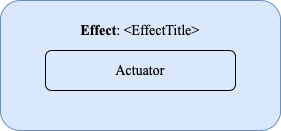
\includegraphics[width=6.5cm]{Figures/Conceptual Model/EffectBlock.png}
	\caption{Effect: graphical representation}
	\label{fig:EffectBlock}
\end{figure}